\documentclass[10pt,twocolumn]{article}
\usepackage[a4paper,margin=18mm,columnsep=7mm]{geometry}
\usepackage[T1]{fontenc}
\usepackage{mathptmx}
\usepackage{microtype}
\usepackage{graphicx}
\usepackage{booktabs}
\usepackage{amsmath,amssymb}
\usepackage{tikz}
\usetikzlibrary{arrows.meta,positioning,fit,calc}
\usepackage[hidelinks]{hyperref}
\usepackage{cleveref}

\newcommand{\VisAMAE}{60.3}\newcommand{\VisARMSE}{96.6}\newcommand{\VisAN}{182}\newcommand{\VisASec}{2.1}
\newcommand{\VisBMAE}{7.7}\newcommand{\VisBRMSE}{12.9}\newcommand{\VisBN}{316}\newcommand{\VisBSec}{2.5}


\title{\vspace{-8mm}\textbf{CrowdSentinel: An Uncertainty-Aware Digital Twin\\for Real-Time Crowd Safety Monitoring}}
\author{Bathri\\
\small School of Computing and Data Science, Sai University, Chennai, India}
\date{}

\begin{document}
\maketitle

\begin{abstract}
Crowd crushes keep occurring at rallies, festivals and concerts, including at events monitored by camera analytics, because dangerous densities often build up where no camera is looking. We present \emph{CrowdSentinel}, a control-room digital twin that fuses CCTV, drone, cell-tower and WiFi observations into a per-zone estimate of crowd density \emph{together with its uncertainty}. A single Kalman filter over all zones of the venue treats every source, including coarse regional counts, as a linear measurement; uncertainty grows wherever no sensor has looked recently. We use this uncertainty twice: to flag zones whose possible density is dangerous but unverified, and to steer a drone towards the location where uncertainty weighted by possible risk is highest. On five simulated rallies of 4{,}000 people generated with a social-force model, the full system lowers zone density error by 73\% relative to a CCTV-only dashboard, and active drone guidance lowers error in camera-free zones by 49\% relative to a fixed patrol. All 25 zones that became critical ($\geq$\,6 persons/m$^2$) were detected, about 69\,s in advance on average, against 3 of 25 for the CCTV-only baseline. The pretrained DM-Count density model used for real video reaches an MAE of \VisAMAE{} on ShanghaiTech Part A and \VisBMAE{} on Part B on a laptop CPU. Code, simulator and experiments are open source.
\end{abstract}

\section{Introduction}
Large gatherings are a recurring source of fatal crowd crushes. Post-incident analyses, such as that of the 2010 Love Parade disaster~\cite{helbing2012love}, show that crushes develop over minutes as density and turbulent pushing build up in bottlenecks, often in areas that organisers cannot see well. Many cities now operate command centres with CCTV analytics, but a camera dashboard reports counts only where cameras point. Its silence about everywhere else is easily read as ``no problem''.

We argue that a crowd-safety system should know \emph{where it is blind}. This paper makes three contributions:
\begin{enumerate}
\item A \textbf{multi-source fusion} formulation in which every source, from a per-zone CCTV count to a cell-tower sector total, is a linear measurement of zone counts. One Kalman filter fuses them and yields a calibrated uncertainty per zone.
\item An \textbf{uncertainty-aware risk layer} that flags zones whose upper density estimate is dangerous even when the best estimate is not, and a short-horizon early-warning rule.
\item \textbf{Active drone guidance} that sends the drone to the footprint with the largest uncertainty weighted by possible risk, discounted by travel time.
\end{enumerate}
Because real ground truth for an entire venue does not exist, we evaluate on a simulated venue where the position of every person is known, and evaluate the vision component separately on a public benchmark. We report the limitations of this setup explicitly (\cref{sec:limits}).

\section{Related work}
\textbf{Crowd counting.} Density-map regression replaced detection for dense scenes after Zhang et al.~\cite{zhang2016mcnn} introduced the ShanghaiTech dataset. CSRNet~\cite{li2018csrnet} and DM-Count~\cite{wang2020dmcount} are widely used single-image models; we use DM-Count with its published weights.

\textbf{Crowd dynamics and safety.} The social-force model~\cite{helbing1995social,helbing2000panic} reproduces pedestrian flows, bottleneck clogging and body compression. Helbing et al.~\cite{helbing2007disasters} identified \emph{crowd pressure}, density times local velocity variance, as a precursor of crowd turbulence. Density levels of service go back to Fruin~\cite{fruin1971} and are standard in crowd-safety practice~\cite{still2014}.

\textbf{Fusion and active sensing.} The Kalman filter~\cite{kalman1960} is the classical tool for fusing noisy linear measurements. Choosing where to sense to reduce uncertainty is studied as sensor placement and informative path planning~\cite{krause2008}. Our contribution is to combine these established tools into a deployable crowd-safety twin and to measure the effect of uncertainty-driven sensing on detection of dangerous zones.

\section{System}
\Cref{fig:arch} shows the architecture and \cref{fig:dash} the operator view. The venue is divided into square zones of 5\,m. Every 2\,s, adapters turn each source into records $(\mathcal{Z}, z, r)$: the people in zone set $\mathcal{Z}$ number $z$ with variance $r$.

\begin{figure}[t]
\centering
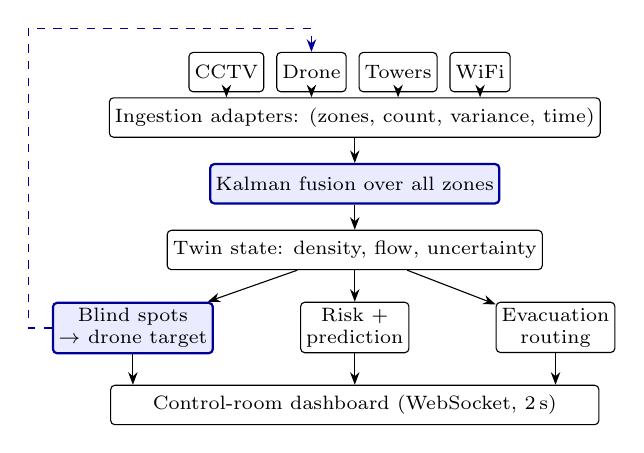
\begin{tikzpicture}[font=\scriptsize, node distance=3.2mm,
  box/.style={draw, rounded corners=1.5pt, align=center, minimum height=5mm, inner sep=2pt},
  hl/.style={box, fill=blue!8, draw=blue!60!black, thick}, ->/.style={-{Stealth[length=1.6mm]}}]
\node[box] (cctv) {CCTV};
\node[box, right=1.5mm of cctv] (drone) {Drone};
\node[box, right=1.5mm of drone] (tower) {Towers};
\node[box, right=1.5mm of tower] (wifi) {WiFi};
\node[box, below=of $(drone)!0.5!(tower)$, minimum width=62mm] (ing) {Ingestion adapters: (zones, count, variance, time)};
\node[hl, below=of ing] (kf) {Kalman fusion over all zones};
\node[box, below=of kf] (state) {Twin state: density, flow, uncertainty};
\node[hl, below left=4mm and -6mm of state] (blind) {Blind spots\\$\rightarrow$ drone target};
\node[box, below=4mm of state] (risk) {Risk +\\prediction};
\node[box, below right=4mm and -6mm of state] (evac) {Evacuation\\routing};
\node[box, below=4mm of risk, minimum width=62mm] (dash) {Control-room dashboard (WebSocket, 2\,s)};
\foreach \s in {cctv,drone,tower,wifi} \draw[->] (\s) -- (\s|-ing.north);
\draw[->] (ing) -- (kf); \draw[->] (kf) -- (state);
\draw[->] (state) -- (blind); \draw[->] (state) -- (risk); \draw[->] (state) -- (evac);
\draw[->] (blind) -- (blind|-dash.north); \draw[->] (risk) -- (dash); \draw[->] (evac) -- (evac|-dash.north);
\draw[->, dashed, blue!60!black] (blind.west) -- ($(blind.west)+(-3mm,0)$) |- ($(drone.north)+(0,3mm)$) -- (drone.north);
\end{tikzpicture}
\caption{Architecture. Highlighted: fusion and the blind-spot module, which closes a loop by moving the drone.}
\label{fig:arch}
\end{figure}

\subsection{Fusion}
Let $\mathbf{x}\in\mathbb{R}^n$ be people counts in the $n$ walkable zones. We use a random-walk process model $\mathbf{x}_k = \mathbf{x}_{k-1} + \mathbf{w}_k$ with spatially correlated noise
\begin{equation}
\mathbf{Q} = \Delta t\, \mathbf{S}\,\mathbf{C}\,\mathbf{S},\qquad \mathbf{C} = \mathrm{norm}(\mathbf{G}\mathbf{G}^\top),
\end{equation}
where $\mathbf{S}=\mathrm{diag}(\sqrt{q_0^2 + (q_1 x_i)^2})$ scales noise with crowd size and $G_{ij}=\exp(-d_{ij}^2/\ell^2)$ links neighbouring zones ($\ell=5$\,m). Building $\mathbf{C}$ as a Gram matrix keeps it positive semi-definite; in our first implementation a truncated Gaussian kernel was not, and the filter diverged once regional measurements were added. Each record contributes a row $\mathbf{h}$ with ones on its zones, so a camera zone count and a tower sector total are handled identically. Delayed reports get extra variance proportional to their delay. We use the Joseph-form update and clip counts at zero only when reporting, because clipping inside the filter biases the estimate upward.

\subsection{Risk, prediction and blind spots}
Zones are graded by density: below 2, 2--4, 4--6 and at least 6 persons/m$^2$ (critical)~\cite{fruin1971,still2014}. With $\sigma_i$ the posterior standard deviation of zone density, a zone is \emph{unverified} when $d_i+\sigma_i$ reaches a higher level than $d_i$. A warning is raised when a zone with $d_i\geq 4.5$ is rising with a smoothed trend that reaches 6 within 120\,s, held for three consecutive ticks.

Every 10\,s the drone, with a 25\,m footprint $\mathcal{F}(p)$, is sent to
\begin{equation}
p^\star = \arg\max_{p}\; \frac{\sum_{i\in\mathcal{F}(p)} \sigma_i^2\,\bigl(1 + 2\min(2, \tfrac{d_i+\sigma_i}{6})\bigr)}{1 + \tau(p)/30\,\mathrm{s}},
\end{equation}
where $\tau(p)$ is the flight time. Evacuation routes come from a Dijkstra search on the zone graph with walls removed and cost growing with density; exits clear at 1.3 persons per metre per second.

\subsection{Real video}
For real cameras, DM-Count~\cite{wang2020dmcount} predicts a density map per frame. A homography from four calibrated points maps each density cell to a ground zone; counts are additive, so they are summed per zone. Farneback optical flow projected through the same homography gives zone velocities and crowd pressure.

\begin{figure*}[t]
\centering
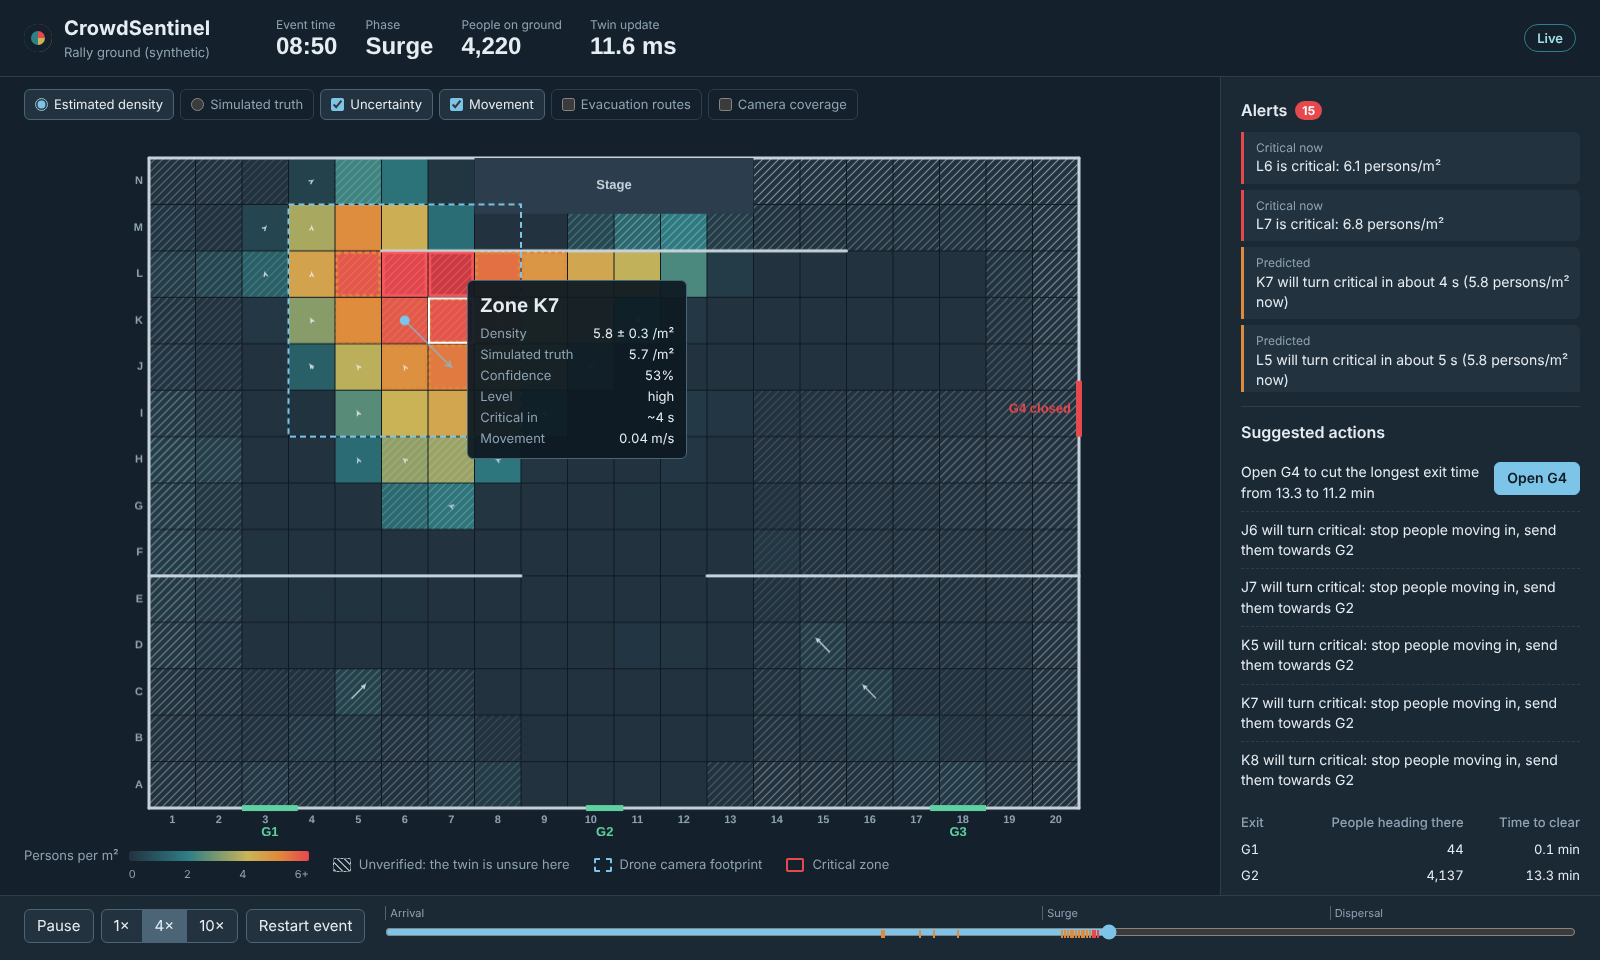
\includegraphics[width=0.92\textwidth]{../dashboard.png}
\caption{Control-room dashboard during the surge. Colour is estimated density; hatching marks zones the twin is unsure about; the dashed square is the drone footprint; red outlines are critical zones. Alerts, suggested actions and exit clearance times are on the right.}
\label{fig:dash}
\end{figure*}

\section{Experimental setup}
\textbf{Venue and crowd.} A 100\,m$\times$70\,m rally ground with a stage, a front barrier, an internal fence with a 20\,m gap, three entry gates and a closed side gate. A social-force simulation (0.05\,s steps) brings in 4{,}000 people over 6 minutes, then a surge pushes towards the stage for 2 minutes and finally everyone leaves. Peak front densities reach about 7 persons/m$^2$. We run 5 random seeds.

\textbf{Sensors.} Four fixed cameras cover the stage centre and right, the fence gap and the middle gate (8\% count error, undercounting above 3 persons/m$^2$, random outages); the stage's front-left is deliberately uncovered. The drone has 12\% error and flies at 6\,m/s. Three cell-tower sectors report phone counts (85\% ownership, background phones) every 10\,s with a 10\,s delay. Four WiFi hotspots (30\% connection rate, 15\,m radius) report every 6\,s.

\textbf{Baselines.} A CCTV-only dashboard (cells without a camera keep their last value), a confidence-weighted fusion, the Kalman filter with CCTV only, and drone policies: hover, random waypoints, fixed lawn-mower patrol and our active policy.

\section{Results}
\Cref{tab:fusion} reports zone density error averaged over the event. Fusion of all sources with the active drone reduces error by 73\% against the CCTV-only dashboard and by 76\% in zones with no camera. The simple weighted fusion does \emph{not} beat CCTV-only on zone error, although it fixes the headcount: spreading sector totals uniformly misplaces people. The Kalman filter exploits the same totals without this problem.

\begin{table}[t]
\centering\small
\caption{Density error (persons/m$^2$, mean over 5 seeds).}
\label{tab:fusion}
\begin{tabular}{@{}lccc@{}}
\toprule
Configuration & All & No camera & Headcount \\
\midrule
CCTV-only dashboard & 0.280 & 0.348 & 63.9\% \\
Weighted fusion, all & 0.307 & 0.375 & 17.2\% \\
Kalman, CCTV only & 0.264 & 0.323 & 47.1\% \\
Kalman, all, patrol & 0.139 & 0.163 & 12.9\% \\
\textbf{Kalman, all, active} & \textbf{0.077} & \textbf{0.083} & \textbf{8.1\%} \\
\midrule
\quad without drone & 0.278 & 0.343 & 13.7\% \\
\quad without towers & 0.070 & 0.074 & 5.9\% \\
\quad without WiFi & 0.077 & 0.084 & 9.4\% \\
\quad without CCTV & 0.105 & 0.089 & 13.1\% \\
\bottomrule
\end{tabular}
\end{table}

\textbf{Ablation.} The drone is the most valuable source in this layout; removing it nearly cancels the gain. Removing cell towers slightly \emph{improves} zone error: their delay and coarse sectors add noise once cameras and the drone cover the crowd. Without CCTV the twin still reaches 0.105, which indicates graceful degradation when cameras fail.

\textbf{Drone guidance.} \Cref{tab:drone} compares policies. The active policy has the lowest error in camera-free zones, 49\% below the fixed patrol. Random waypoints are a strong baseline for catching dangerous zones (both about 87\%), but the active policy is more accurate.

\begin{table}[t]
\centering\small
\caption{Drone policies (Kalman, all sources).}
\label{tab:drone}
\begin{tabular}{@{}lcc@{}}
\toprule
Policy & Error, no camera & Zones $\geq 4$ caught \\
\midrule
Hover at centre & 0.326 & 37.7\% \\
Random waypoints & 0.113 & 86.7\% \\
Fixed patrol & 0.163 & 68.8\% \\
\textbf{Active (ours)} & \textbf{0.083} & \textbf{86.5\%} \\
\bottomrule
\end{tabular}
\end{table}

\textbf{Early warning.} Across seeds, 25 zones truly became critical. The CCTV-only dashboard detected 3 of them, because the surge peaks in the uncovered front-left. The full twin raised a threshold alarm for 21 with 100\% precision, and with prediction it detected all 25 a mean $69\pm14$\,s before the crossing, at 41\% alarm precision. Prediction therefore buys about a minute of warning at the cost of more false alarms; operators can choose either operating point.

\textbf{Latency.} One full twin update takes 26\,ms on average (Python, CPU), far below the 2\,s update interval.

\begin{figure}[t]
\centering
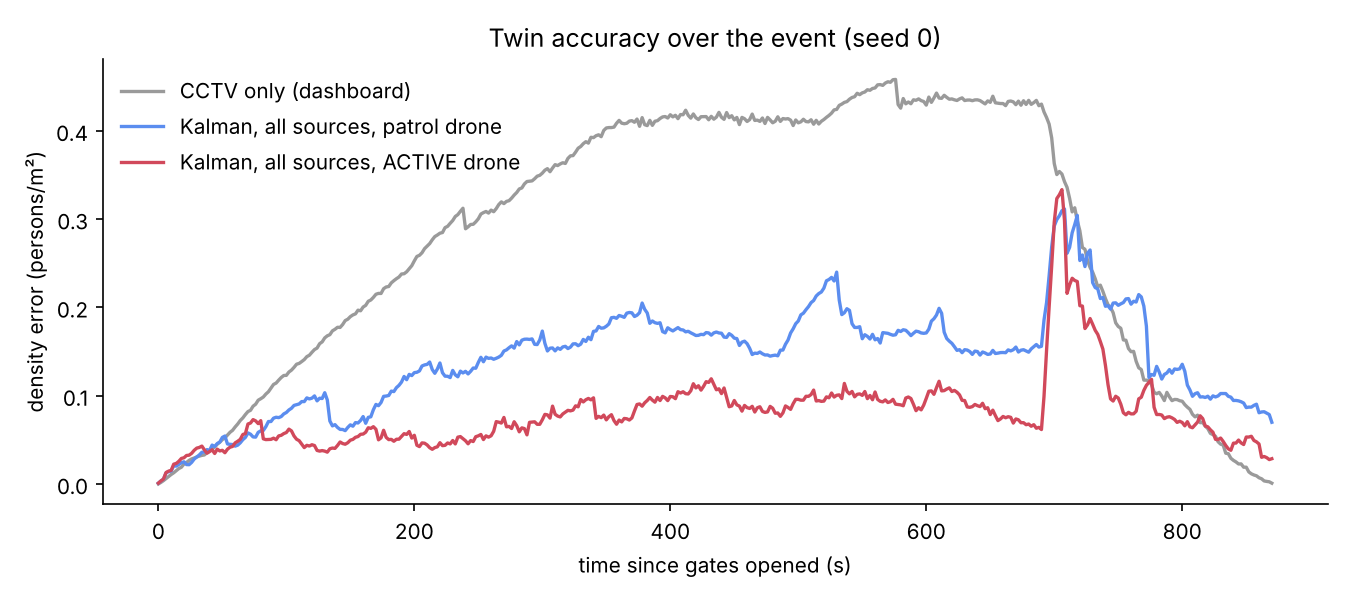
\includegraphics[width=\columnwidth]{../../experiments/results/error_over_time.png}
\caption{Density error over one event (seed 0). The fused twin lags for about a minute when dispersal begins at 690\,s.}
\label{fig:time}
\end{figure}

\textbf{Vision.} \Cref{tab:vision} reports DM-Count with the authors' weights on the official ShanghaiTech test sets, run on a laptop CPU through our pipeline. Errors are close to the published MAE of 59.7 (Part A) and 7.4 (Part B)~\cite{wang2020dmcount}, which confirms that the integration (preprocessing, weights, ground-truth parsing) is correct. At about 2\,s per image on CPU, a GPU or a lighter model is needed to process many camera feeds at 2 frames per second.

\begin{table}[t]
\centering\small
\caption{DM-Count on ShanghaiTech test sets (people per image).}
\label{tab:vision}
\begin{tabular}{@{}lcccc@{}}
\toprule
Part & Images & MAE & RMSE & s/image (CPU) \\
\midrule
A (dense) & \VisAN & \VisAMAE & \VisARMSE & \VisASec \\
B (sparse) & \VisBN & \VisBMAE & \VisBRMSE & \VisBSec \\
\bottomrule
\end{tabular}
\end{table}

\section{Limitations}\label{sec:limits}
Ground truth, tower and WiFi data are simulated; real feeds need telecom and venue partnerships. Results come from one venue and one camera layout chosen to contain a blind spot, so absolute numbers should not be generalised. Prediction parameters were tuned on one of the five evaluation seeds. The random-walk process model reacts slowly to sudden collective movement (\cref{fig:time}); a forecast that runs the crowd model forward from the fused state is the natural next step. The system supports human decisions and performs no identification of individuals.

\section{Conclusion}
CrowdSentinel shows that treating uncertainty as a first-class output changes what a crowd-safety twin can detect: the zones that turned critical in our scenarios were exactly the ones a camera dashboard could not see, and uncertainty-driven drone guidance found them. Next steps are validation on recorded real events and simulation-based forecasting.

\begin{thebibliography}{99}\small
\bibitem{helbing2012love} D.~Helbing and P.~Mukerji, ``Crowd disasters as systemic failures: analysis of the Love Parade disaster,'' \emph{EPJ Data Science}, 1:7, 2012.
\bibitem{zhang2016mcnn} Y.~Zhang, D.~Zhou, S.~Chen, S.~Gao, and Y.~Ma, ``Single-image crowd counting via multi-column convolutional neural network,'' in \emph{CVPR}, 2016.
\bibitem{li2018csrnet} Y.~Li, X.~Zhang, and D.~Chen, ``CSRNet: Dilated convolutional neural networks for understanding the highly congested scenes,'' in \emph{CVPR}, 2018.
\bibitem{wang2020dmcount} B.~Wang, H.~Liu, D.~Samaras, and M.~Hoai, ``Distribution matching for crowd counting,'' in \emph{NeurIPS}, 2020.
\bibitem{helbing1995social} D.~Helbing and P.~Moln\'ar, ``Social force model for pedestrian dynamics,'' \emph{Physical Review E}, 51(5):4282--4286, 1995.
\bibitem{helbing2000panic} D.~Helbing, I.~Farkas, and T.~Vicsek, ``Simulating dynamical features of escape panic,'' \emph{Nature}, 407:487--490, 2000.
\bibitem{helbing2007disasters} D.~Helbing, A.~Johansson, and H.~Z.~Al-Abideen, ``Dynamics of crowd disasters: an empirical study,'' \emph{Physical Review E}, 75:046109, 2007.
\bibitem{fruin1971} J.~J.~Fruin, \emph{Pedestrian Planning and Design}. Metropolitan Association of Urban Designers and Environmental Planners, 1971.
\bibitem{still2014} G.~K.~Still, \emph{Introduction to Crowd Science}. CRC Press, 2014.
\bibitem{kalman1960} R.~E.~Kalman, ``A new approach to linear filtering and prediction problems,'' \emph{Journal of Basic Engineering}, 82(1):35--45, 1960.
\bibitem{krause2008} A.~Krause, A.~Singh, and C.~Guestrin, ``Near-optimal sensor placements in Gaussian processes: theory, efficient algorithms and empirical studies,'' \emph{JMLR}, 9:235--284, 2008.
\end{thebibliography}

\end{document}
